\documentclass[11pt]{article}
\usepackage{geometry}                % See geometry.pdf to learn the layout options. There are lots.
\geometry{letterpaper}                  % ... or a4paper or a5paper or ... 
%\geometry{landscape}                % Activate for for rotated page geometry
%\usepackage[parfill]{parskip}    % Activate to begin paragraphs with an empty line rather than an indent
\usepackage{graphicx}
\usepackage{amssymb}
\usepackage{epstopdf}
\usepackage{multicol}
\DeclareGraphicsRule{.tif}{png}{.png}{`convert #1 `dirname #1`/`basename #1 .tif`.png}

\title{Physics 250 Lab \#1}
\author{Avery Karlin, Colin Christie, and Ryan Greenberg}
\date{January 24, 2017}                                           

\begin{document}


\maketitle
\begin{abstract} This lab covers the Millikan Oil-Drop Experiment, attempting to recreate the precise measurement of the electric charge quanta that won Millikan the Nobel Prize in 1923.
\end{abstract}
%\begin{twocolumn}

\section{Introduction}
The charge of an electron and the discrete electric quanta was one of the most fundamental result of atomic physics, using a microscope chamber with oil droplets inside, achieving terminal downward velocity by gravitational force. By using electric potential inside the measurement, it can be forced upwards against gravity, using the dynamics of the drop to calculate the electric force acting on it, and determine the charge of the particle.

\section{Apparatus}
The oil is sprayed into the reservoir using an atomizer, viewed by a microscope going to the viewing chamber made up of metal plates, with glass on the sides to allow visibility, acting as a large capacitor. The viewing chamber illuminated by an angled lamp, with a focusing lens and a heat absorbing glass to prevent air currents from the lamp heat. While the drops themselves are not visible, the reflection of the light off of the drops is visible, appearing as bright drops on the dim background given by the angled lamp. The capacitor is connected to a voltage producing device at 300 V, with a tri-state switch to control the direction of the voltage and if it is on, such that when an oil drop is seen, it can be suspended using the voltage, allowing measurement of the charge.

\begin{figure}[h]
\begin{center}
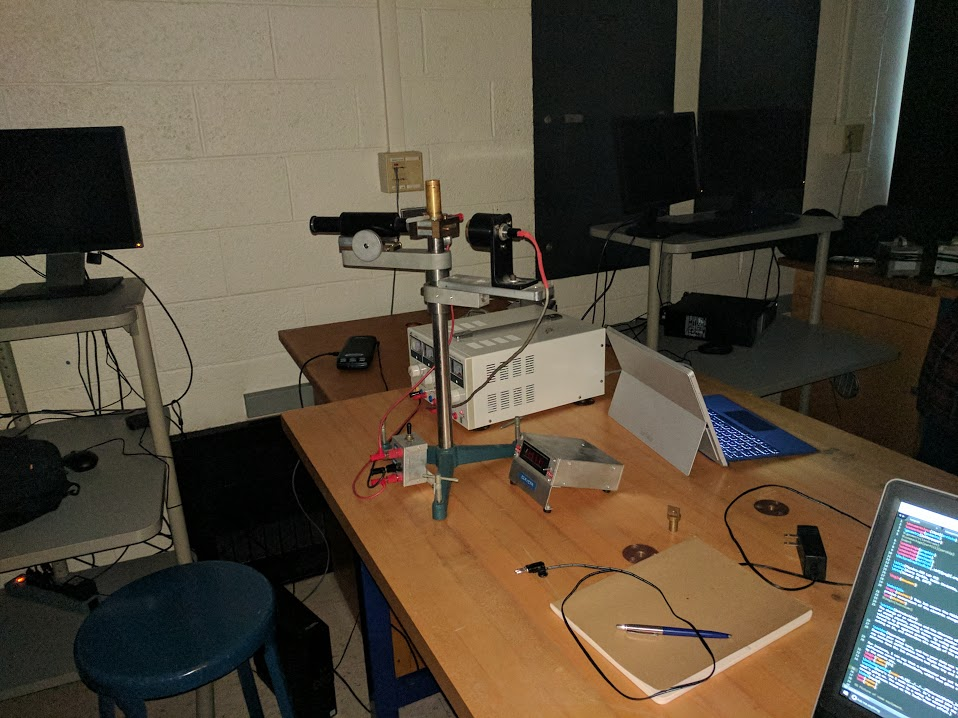
\includegraphics[scale=0.4]{lab1.jpg}
\caption{This is the photo of the setup of the experiment, especially the microscope with the viewing chamber and the voltage producing device.}
\label{equip}
\end{center}
\end{figure}

\section{Measurements/Data} \label{Measurements}

\begin{table}[htp]
\begin{center}
\begin{tabular}{|c|c|c|c|c|}
\hline
Metric & Drop 1 & Drop 2 & Drop 3 & Drop 4 \\ \hline
Rising Time 1 (s) & 1.83 & 3.33 & 5.33 & 1.39 \\
Rising Time 2 (s) & 1.89 & 3.28 & 5.64 & 1.26 \\
Rising Time 3 (s) & 1.94 & 3.56 & 5.3 & 1.37 \\
Falling Time 1 (s) & 13.88 & 9.68 & 12.15 & 11.24 \\
Falling Time 2 (s) & 15.43 & 9.85 & 12.76 & 13.77 \\
Falling Time 3 (s) & 19.28 & 8.02 & 13.29 & 12.96 \\ 
Average Rising Distance (m) & 0.00032 & 0.00032 & 0.00032 & 0.00032 \\
Average Falling Distance (m) & 0.00032 & 0.00032 & 0.00032 & 0.00032 \\
\hline
\end{tabular}
\caption{Measured Data}
\end{center}
\label{table}
\end{table}

\section{Analysis}

The average of the rising distances and falling distances combined with the times are used to calculate the average rising and falling velocity for each drop. The radius can be calculated the equation, $r = 9.66 * 10^{-5} \sqrt{v_f}$. Using the equation $q\frac{V}{d} = K\sqrt{v_f}(v_f + v_r)(1 + \frac{8.23 * 10^{-8}}{r})^{-\frac{3}{2}}$ as a correction to Stoke's Law, which states that $q\frac{V}{d} = K\sqrt{v_f}(v_f + v_r)$, the charge of the droplets can be calculated as a result.

\begin{table}[htp]
\begin{center}
\begin{tabular}{|c|c|c|c|c|}
\hline
Metric & Drop 1 & Drop 2 & Drop 3 & Drop 4 \\ \hline
Average Rising Velocity (m/s) & 0.000169611 & 5.90043E-05 & 9.43953E-05 & 0.000238806 \\
Average Falling Velocity (m/s) & 1.97572E-05 & 3.48457E-05 & 2.51309E-05 & 2.52831E-05 \\
Radius (m) & 4.29378E-07 & 5.70232E-07 & 4.84263E-07 & 4.85727E-07 \\
Integer Multiple of e & 2 & 2 & 1 & 3 \\
Charge (C) & 3.44745E-19 & 3.32058E-19 & 1.77581E-19 & 5.59455E-19 \\
Calculated Value of e (C) & 1.72373E-19 & 1.66029E-19 & 1.77581E-19 & 1.86485E-19 \\ \hline
\end{tabular}
\caption{Calculated Data}
\end{center}
\label{table2}
\end{table}

\begin{figure}[h]
\begin{center}
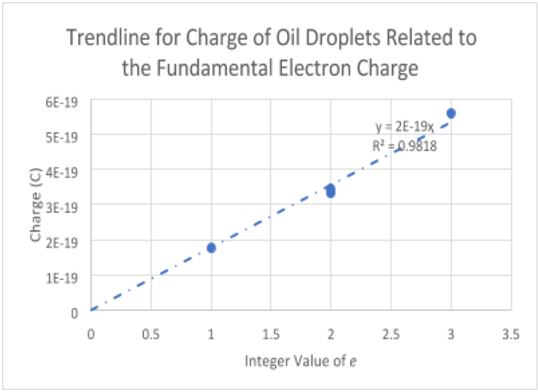
\includegraphics[scale=1]{PhysicsLab1.jpg}
\label{equip}
\end{center}
\end{figure}

\section{Conclusions}

Assuming that the accepted charge for an electron is 1.602 × 10-19 C, only the value of e calculated from the results of Drop 2 is within the margin of uncertainty defined by the standard deviation. The experimental values are nevertheless surprisingly close to the accepted value of e (the value for Drop 1 is off by 7.62\%, Drop 2 by 3.62\%, Drop 3 by 10.8\%, and Drop 4 by 16.4\%) given the considerable potential for error in the experiment. The most likely error ought to be the inevitable delay caused by human reaction time in using the stopwatch. The errors introduced by delayed reaction would give less accurate values for the times it took the oil droplets to travel given distances, and consequently lead to errant values for velocity and in turn faulty calculations for charge. Another possible error would be the failure to notice or account for a change in velocity during the timing of a rising droplet of oil. In the electric field, an increase in velocity implies a gain of charge, and a decrease in velocity implies a loss of charge. Failure to account for a sudden change in velocity during the time of measurement implies a failure to account for a change in charge during the time of measurement, which would ultimately lead to a calculated value for charge between 2 multiples of e, which is understood not to be possible. Other possible sources of error include the loss of electromotive force to internal resistance, which would lead to an inaccurate value of V in the equation used to calculate charge; and failure to account for the change in the permittivity of the capacitor when the reservoir is placed inside, which would introduce the need for an adjusted constant in the equation to describe the system accurately.

The calculated standard deviation of the value of e as a result is 7.4903E-21, with an average value e of 1.75617E-19 C, for a percent error of 9.62\%.
%\end{twocolumn}
\end{document}  